%!TEX TS-program = xelatex

% Author: Georgy Perevozchikov (gosha20777@live.com)
% https://github.com/gosha20777/bachelor-diploma

\documentclass[a4paper,14pt]{extarticle} % 14й шрифт
%%% Преамбула %%%

\usepackage{fontspec} % XeTeX
\usepackage{xunicode} % Unicode для XeTeX
\usepackage{xltxtra}  % Верхние и нижние индексы
\usepackage{pdfpages} % Вставка PDF

\usepackage{listings} % Оформление исходного кода
\lstset{
    basicstyle=\small\ttfamily, % Размер и тип шрифта
    breaklines=true, % Перенос строк
    tabsize=2, % Размер табуляции
    literate={--}{{-{}-}}2 % Корректно отображать двойной дефис
}

% Шрифты, xelatex
\defaultfontfeatures{Ligatures=TeX}
\setmainfont{Times New Roman} % Нормоконтроллеры хотят именно его
\newfontfamily\cyrillicfont{Times New Roman}
%\setsansfont{Liberation Sans} % Тут я его не использую, но если пригодится
\setmonofont{FreeMono} % Моноширинный шрифт для оформления кода

% Русский язык
\usepackage{polyglossia}
\setdefaultlanguage{russian}

\usepackage{amssymb,amsfonts,amsmath} % Математика
\numberwithin{equation}{section} % Формула вида секция.номер

\usepackage{enumerate} % Тонкая настройка списков
\usepackage{indentfirst} % Красная строка после заголовка
\usepackage{float} % Расширенное управление плавающими объектами
\usepackage{multirow} % Сложные таблицы

% Пути к каталогам с изображениями
\usepackage{graphicx} % Вставка картинок и дополнений
\graphicspath{{images/}{images/userguide/}{images/testing/}{images/infrastructure/}{extra/}{extra/drafts/}}

% Формат подрисуночных записей
\usepackage{chngcntr}
\counterwithin{figure}{section}

% Гиперссылки
\usepackage{hyperref}
\hypersetup{
    colorlinks, urlcolor={black}, % Все ссылки черного цвета, кликабельные
    linkcolor={black}, citecolor={black}, filecolor={black},
    pdfauthor={Георгий Перевозчиков},
    pdftitle={Разработка моделей глубокого машинного обучения для распознования людей по аэрофотоснимкам в Поисково-Спасательных Операциях}
}

% Оформление библиографии и подрисуночных записей через точку
\makeatletter
\renewcommand*{\@biblabel}[1]{\hfill#1.}
\renewcommand*\l@section{\@dottedtocline{1}{1em}{1em}}
\renewcommand{\thefigure}{\thesection.\arabic{figure}} % Формат рисунка секция.номер
\renewcommand{\thetable}{\thesection.\arabic{table}} % Формат таблицы секция.номер
\def\redeflsection{\def\l@section{\@dottedtocline{1}{0em}{10em}}}
\makeatother

\renewcommand{\baselinestretch}{1.4} % Полуторный межстрочный интервал
\parindent 1.27cm % Абзацный отступ

\sloppy             % Избавляемся от переполнений
\hyphenpenalty=1000 % Частота переносов
\clubpenalty=10000  % Запрещаем разрыв страницы после первой строки абзаца
\widowpenalty=10000 % Запрещаем разрыв страницы после последней строки абзаца

% Отступы у страниц
\usepackage{geometry}
\geometry{left=3cm}
\geometry{right=1cm}
\geometry{top=2cm}
\geometry{bottom=2cm}

% Списки
\usepackage{enumitem}
\setlist[enumerate,itemize]{leftmargin=12.7mm} % Отступы в списках

\makeatletter
    \AddEnumerateCounter{\asbuk}{\@asbuk}{м)}
\makeatother
\setlist{nolistsep} % Нет отступов между пунктами списка
\renewcommand{\labelitemi}{--} % Маркет списка --
\renewcommand{\labelenumi}{\asbuk{enumi})} % Список второго уровня
\renewcommand{\labelenumii}{\arabic{enumii})} % Список третьего уровня

% Содержание
\usepackage{tocloft}
\renewcommand{\cfttoctitlefont}{\hspace{0.38\textwidth}\MakeTextUppercase} % СОДЕРЖАНИЕ
\renewcommand{\cftsecfont}{\hspace{0pt}}            % Имена секций в содержании не жирным шрифтом
\renewcommand\cftsecleader{\cftdotfill{\cftdotsep}} % Точки для секций в содержании
\renewcommand\cftsecpagefont{\mdseries}             % Номера страниц не жирные
\setcounter{tocdepth}{3}                            % Глубина оглавления, до subsubsection

% Нумерация страниц справа сверху
\usepackage{fancyhdr}
\pagestyle{fancy}
\fancyhf{}
\fancyhead[R]{\textrm{\thepage}}
\fancyheadoffset{0mm}
\fancyfootoffset{0mm}
\setlength{\headheight}{17pt}
\renewcommand{\headrulewidth}{0pt}
\renewcommand{\footrulewidth}{0pt}
\fancypagestyle{plain}{ 
    \fancyhf{}
    \rhead{\thepage}
}

% Формат подрисуночных надписей
\RequirePackage{caption}
\DeclareCaptionLabelSeparator{defffis}{ -- } % Разделитель
\captionsetup[figure]{justification=centering, labelsep=defffis, format=plain} % Подпись рисунка по центру
\captionsetup[table]{justification=raggedright, labelsep=defffis, format=plain, singlelinecheck=false} % Подпись таблицы слева
\addto\captionsrussian{\renewcommand{\figurename}{Рис.}} % Имя фигуры

% Пользовательские функции
\newcommand{\addimg}[4]{ % Добавление одного рисунка
    \begin{figure}
        \centering
        \includegraphics[width=#2\linewidth]{#1}
        \caption{#3} \label{#4}
    \end{figure}
}
\newcommand{\addimghere}[4]{ % Добавить рисунок непосредственно в это место
    \begin{figure}[H]
        \centering
        \includegraphics[width=#2\linewidth]{#1}
        \caption{#3} \label{#4}
    \end{figure}
}
\newcommand{\addtwoimghere}[5]{ % Вставка двух рисунков
    \begin{figure}[H]
        \centering
        \includegraphics[width=#2\linewidth]{#1}
        \hfill
        \includegraphics[width=#3\linewidth]{#2}
        \caption{#4} \label{#5}
    \end{figure}
}
\newcommand{\addimgapp}[2]{ % Это костыль для приложения Б
    \begin{figure}[H]
        \centering
        \includegraphics[width=1\linewidth]{#1}
        \caption*{#2}
    \end{figure}
}

% Заголовки секций в оглавлении в верхнем регистре
\usepackage{textcase}
\makeatletter
\let\oldcontentsline\contentsline
\def\contentsline#1#2{
    \expandafter\ifx\csname l@#1\endcsname\l@section
        \expandafter\@firstoftwo
    \else
        \expandafter\@secondoftwo
    \fi
    {\oldcontentsline{#1}{\MakeTextUppercase{#2}}}
    {\oldcontentsline{#1}{#2}}
}
\makeatother

% Оформление заголовков
\usepackage[compact,explicit]{titlesec}
\titleformat{\section}{}{}{12.5mm}{\centering{\thesection\quad\MakeTextUppercase{#1}}\vspace{1.5em}}
\titleformat{\subsection}[block]{\vspace{1em}}{}{12.5mm}{\thesubsection\quad#1\vspace{1em}}
\titleformat{\subsubsection}[block]{\vspace{1em}\normalsize}{}{12.5mm}{\thesubsubsection\quad#1\vspace{1em}}
\titleformat{\paragraph}[block]{\normalsize}{}{12.5mm}{\MakeTextUppercase{#1}}

% Секции без номеров (введение, заключение...), вместо section*{}
\newcommand{\anonsection}[1]{
    \phantomsection % Корректный переход по ссылкам в содержании
    \paragraph{\centerline{{#1}}\vspace{1.5em}}
    \addcontentsline{toc}{section}{\uppercase{#1}}
}

% Секции для приложений
\newcommand{\appsection}[1]{
    \phantomsection
    \paragraph{\centerline{{#1}}}
    \addcontentsline{toc}{section}{\uppercase{#1}}
}

% Библиография: отступы и межстрочный интервал
\makeatletter
\renewenvironment{thebibliography}[1]
    {\section*{\refname}
        \list{\@biblabel{\@arabic\c@enumiv}}
           {\settowidth\labelwidth{\@biblabel{#1}}
            \leftmargin\labelsep
            \itemindent 16.7mm
            \@openbib@code
            \usecounter{enumiv}
            \let\p@enumiv\@empty
            \renewcommand\theenumiv{\@arabic\c@enumiv}
        }
        \setlength{\itemsep}{0pt}
    }
\makeatother

\setcounter{page}{4} % Начало нумерации страниц
 % Подключаем преамбулу

%%% Начало документа
\begin{document}

%\includepdf{pz} % Пояснительная записка
%\includepdf[pages={1,2}]{task} % Задание на диплом печатается на одном листе с двух сторон
%помимо ПЗ и задания, в диплом также вкладывается отзыв руководителя и рецензия

\tableofcontents % Содержание 
%\clearpage

\anonsection{Введение}

В XXI веке роль технологий обучения и AI (англ. artificial intelligence -- искуственный интеллект) трудно переоценить. Благодоря им значительно упрощается обработка больших данных, люди могут предсказывать события, автоматизировать рпроизводственные процессы, делать новые научне открытия, и решают множество других задач и решать другие важные для человека задачи.

Одной из областей машинного обучения яаляется CV (англ. Compurer Vision -- компьютерное зение). CV позволяет обрабатывать с помощью сверточных нейронных сетей изображения или видео и на основе их анализа делать различные заключения. Благодоря этой технологии время необходимое на обработку таких данных значительно сокращается а человек избавляется от выполнения рутиной работы. Также невилируется фактор усталости человека при выполнении ручной обработки данных, что зачастую приводит к повышению качества выполнения задачи.

Отдельной областью применения является поиск пропавших или потерявшихся людей в природной зоне. В воследнее время для анализа местности все чаще применяются БПЛА (Беспилотные Летательные Аппараты) для проведения аэрофотосъемки. Процесс анализа таких изображений довольно трудоемкий для человека, по этому его можно автоматизировать с помощью технологий компьютерного зрания (CV). 

В описанном в данной работе исследовании приводится мехонизм решения описаной выше проблемы с применением современных технологий компьютерного зрения. Использование сверточных нейронных сетей сопсобно в короткие сроки решить задачу детектирования и локализации пропаышего человека на местности, что нередко может спасти ему жизнь. 

Цель работы -- исследование и разаработка различных архитектур СНС (сверточных нейронных сетей) решающих задачу детектирования потерявшихся в лесу людей по аэрофотоснимкам полученных с БПЛА, разработка пользовательского ПО (Программного Обеспечения) реализующего данную технологию с целью возможного внедрения в ПСО (поисково-спасательные отряды) для непосредственного применения. В разделе 1 описывается проблемы поиска пропаыших в лесу людей и их детектирования по аэрофотоснимкам. В резделе 2 описаны современные методы анализа изображений, принципы работы сверточных нейронных сетей и метрики их оценивания. В разделе 3 изложен процесс обора и подготовки данных для обучения нейросетевых алгоритмов. В разделе 4 производится сравнение раздичных архитектур СНС и объясняется выбор архитектуры RetinaNet-Resnet50. В разделе 5 приводится подробное описание архитектуры RetinaNet-Resnet50. В разделе 6 описан процесс обучения RetinaNet-Resnet50, исследования, улучшающие качество распознования (FPN-shift и Deep FPN), и приведены результаты экспериментов. В разделе 7 приведено пользовательского ПО. В разделе 8 приведены результаты использования данного ПО в различных ПСО.
\clearpage % Введение
\section{Проблема поиска пропавших людей}\label{sect-1}

Неподготовленный человек, попавший в природную среду, может легко заблудиться и пропасть. Достаточно часто люди уходят на природу, в лес -- за грибами, с прогулочными или иными целями -- теряют ориентиры, после чего самостоятельно выбраться из природных условий становится проблематично.

Розыском таких пропавших людей занимаются как и государственные структуры (МЧС, полиция), так и волонтёры в составе Поисково-Спасательных Отрядов (ПСО). Так, например, в России наиболее известными ПСО являются "Лиза Алерт", "Экстремум", "Сова", "Запад", "Орен Спас". Подобные организации распространены и в других странах по всему миру.

Так, по приблизительным оценкам в России каждый год пропадает более ста двадцати тысяч человек, в США -- более ста тысяч, на территории стран Европейского Союза эта цифра составляет приблизительно девяноста тысяч человек.

\subsection{Основные факторы риска потерявшегося человека в природной зоне}

Положение потерявшегося человека часто усугубляется из-за физических и психологических факторов, таких как:

\begin{itemize}
    \item Обезвоживание. Отсутствие доступа к питьевой воде или ограниченный её запас резко снижает возможность человека поддерживать своё стабильное состояние на протяжении длительного времени, которое может потребоваться на проведение спасательной операции;
    \item Гипотермия (переохлаждение). Зимой и в ночное время температура окружающей среды снижается (особенно в природных условиях), а у потерявшегося человека, как правило, нет возможности согреться (если нет соответствующего снаряжения). Данная причина является одной из наиболее частых причин гибели потерявшихся людей;
    \item Травмаы. Человек, который потерялся на природе, нередко начинает паниковать, что приводит к необдуманным, импульсивным поступкам, которые нередко приводят к травмам, после получения которых шансы самостоятельно добраться до цивилизации драматически уменьшаются;
    \item Паника. Осознание потерявшимся факта невозможности самостоятельно выбраться из локации нередко приводит к панике, что резко снижает вероятность успешного выхода потерявшегося человека к цивилизации.
\end{itemize}

Эти и многие другие факторы резко снижают время выживания потерявшегося человека в лесу, что в свою очередь повышает требования к временному ресурсу для поисково-спасательных операций. В среднем потерявшейся человек может продержаться в лесу в течении 6-8 дней, летом и 2-4 дней зимой. Стоит также учесть, что поиск человека может начаться не сразу, а спустя какое-то время. Иными словами -- часто счет идет на часы.
\subsubsection{Основные методики поиска пропавших людей}

Наиболее распространенным способом поиска потерявшегося человека в природной локации является наземная поисковая операция. Это, как правило, пеший поиск с участием ответственных за подобные мероприятия служб или силами волонтёров. 

Район поиска делится на квадраты размером 500$\times$500 метров, и прочесывается отрядом спасателей по заранее оговоренному маршруту (как правило цепью), с целью постараться увидеть или получить отклик потерявшегося человека. 

Данный способ поиска является несомненно точным, но достаточно тяжелым -- необходимо большое количество подготовленных к задаче поиска людей, необходима организация поисковых групп, необходимо выполнение многих других смежных задач. Помимо прочего, пеший поиск является достаточно медленным. Поисковый квадрат размером в лесной зоне закрывается пешей поисковой группой в среднем за 3-6 часов (а таких квадратов может быть несколько).

Другим способом поиска является поиск по фотографиям, с полученных с БПЛА. В последнее время появились небольшие БПЛА и их все чаще применяют спасатели для проведения поисковых работ. 

Над районом поиска составляется маршрут, по которому затем пролетает летательный аппарат, в заранее заданных точках делает фотографии с гео-меткой. После выполнения полётного задания БПЛА возвращается в поисковый штаб, где его оператор меняет на нём аккумулятор и карту памяти со снимками, после чего, загружает следующее полётное задание и дрон отправляется на дальнейшие съёмки с воздуха.

Опытным путём было установлено, что наиболее оптимальная высота для осуществления аэрофотосъёмки региона поиска приблизительно 50 метров. Данная отметка выше крон деревьев, при этом позволяет получить достаточно чёткие фотоснимки, на которых можно заметить человека.

С одной поисковой операции в среднем набирается около четырех тысяч фотографий. Полученные фотографии анализируются специалистами из ГПА (группа просмотра и анализа) с целью найти на них человека. Человек на такой фотографии может быть частично закрыт растительностью и занимает очень мало места -- в среднем взрослый лежачий человек имеет 100 пикселей в высоту и 30 в ширину при исходном размере изображения 4000$\times$3000 пикселей. Это усложняет ручной анализ изображений и пагубно сказывается на усталости анализирующего человека. В среднем опытный специалист из ГПА тратит на анализ одной фотографии около минуты, а его концентрации внимания хватает на анализ 50-70 снимков, после чего, человеку необходим отдых. На анализ четырех тысяч фотографий (одна поисковая операция) у ГПА из 5-6 человек тратится около 6.5 часов.
\subsubsection{Постановка задачи}

Цель работы заключается в исследовании и разработке различных архитектур СНС, решающих задачу детектирования потерявшихся в лесу людей по аэрофотоснимкам полученных с БПЛА, разработке пользовательского ПО, реализующего данную технологию, с целью возможного внедрения в ПСО для непосредственного применения.

В исследовании ведется учет следующих критериев:
\begin{itemize}
    \item Точность алгоритма распознавания -- СНС должна точно находить людей, не пропускать их, а число ложных срабатываний должно быть минимальным;
    \item Скорость алгоритма распознавания -- СНС должна быстро анализировать снимки на персональных компьютерах;
    \item Потребление памяти -- количество потребляемой памяти (зависит от числа параметров СНС и количества ее слоев) должно позволять запускать СНС на персональных компьютерах.
\end{itemize}

Для реализации поставленной цели были сформулированы следующие задачи:
\begin{itemize}
    \item Сбор, анализ и подготовка исходных данных необходимых для обучения нейросетевых математических моделей;
    \item Выбор оптимальной архитектуры нейросетевой модели, проверка возможности ее улучшения, обучение модели;
    \item Проведение оптимизационных работ с целью уменьшение времени работы выбранного нейросетевого алгоритма на ЭВМ;
    \item Разработка интерфейса пользователя;
\end{itemize}

\clearpage % Постановка задачи
\section{Сверточные нейронные сети для решения основных задач компьютерного зрения}

Сверточные нейронные сети (СНС) -- открытые Яном ЛеКуном -- сейчас широко применяются в широком спектре задач анализа изображений. Успех обусловлен возможностью учета двумерной топологии изображения и устойчивости к различным искажениям изображения (изменениям масштаба и кантрастности, смещениям, поворотам и т.д.) в отличие от многослойного персептрона.

На данный момент сверточная нейронная сеть и ее модификации стремительно развиваются и считаются лучшими по точности и скорости алгоритмами нахождения объектов на сцене. Начиная с 2012 года, нейросети занимают первые места на известном международном конкурсе по распознаванию образов ImageNet, во многом обгоняя человека.
\addimghere{2-imagenet-statistics}{1}{Статистика ошибок, совершенных в процессе анализа данных ImageNet за 2010—2015}{imagenet-stat}

dd

\clearpage % Постановка задачи
\section{Сбор и подготовка данных}

Для решения поставленной задачи первоначально был проведен опрос операторов БПЛА из ПСО "Лиза Алерт", и получены несколько примеров снимков. В результате были выяснены следующие аспекты:

\begin{itemize}
    \item Условия съемки:
    \begin{itemize}
        \item Высота -- 40-50 метров над поверхностью земли;
        \item Съемка производиться вертикально (вид сверху);
        \item Во время съемки БПЛА зависает над сценой, чтобы сфокусироваться;
    \end{itemize}
    \item Позы, в которых чаще всего находят потерявшихся людей:
    \begin{itemize}
        \item Стоящий человек (идущий, бегущий);
        \item Сидячий человек (на корточках);
        \item Лежачий человек (на спине);
        \item Лежачий человек (на животе);
        \item Лежачий человек (на боку);
        \item Лежачий в позе эмбриона человек.
    \end{itemize}
\end{itemize}

При поиске доступных открытых решений удалось найти 2 набора данных (dataset-а): SDD (Stanford Drone Dataset) \cite{lib-sdd} и VisDrone DET dataset \cite{lib-visdrone}, но ни один из них не подходил для решения поставленной задачи (рис. \ref{sdd-visdrone-example}). В этих наборах данных несколько отличались условия съемки, а также, отсутствовали, как природная среда, так и интересующие нас позы. Однако, у них есть одно существенное преимущество -- они открыты и довольно распространены, а также, по схожести задачи они значительно ближе, чем какие-либо другие наборы данных. По этому, в описанных ниже исследованиях они использовались для предобучения моделей (а как следствие и сужения доменной области) и оценки качества моделей \cite{lib-transfer-learning}. Также, открытость этих данных и их известность позволила сравнивать качество полученных моделей с уже имеющимися.

\begin{figure}[H]
    \centering
    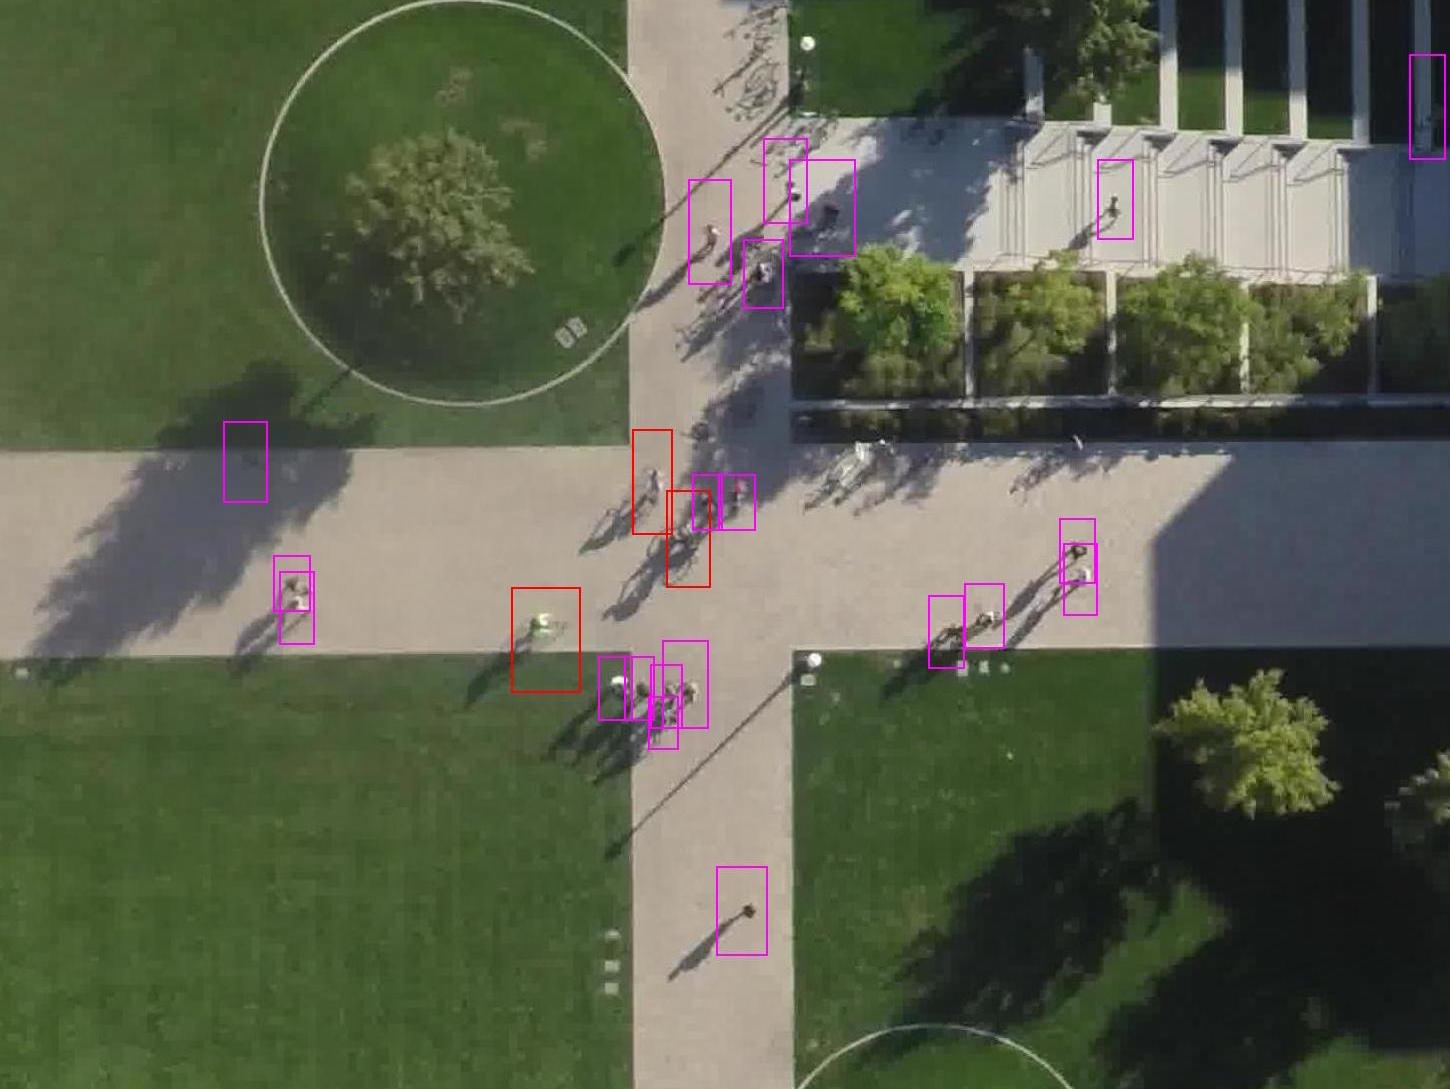
\includegraphics[width=0.42\linewidth]{3-sdd-example}
    \hfill
    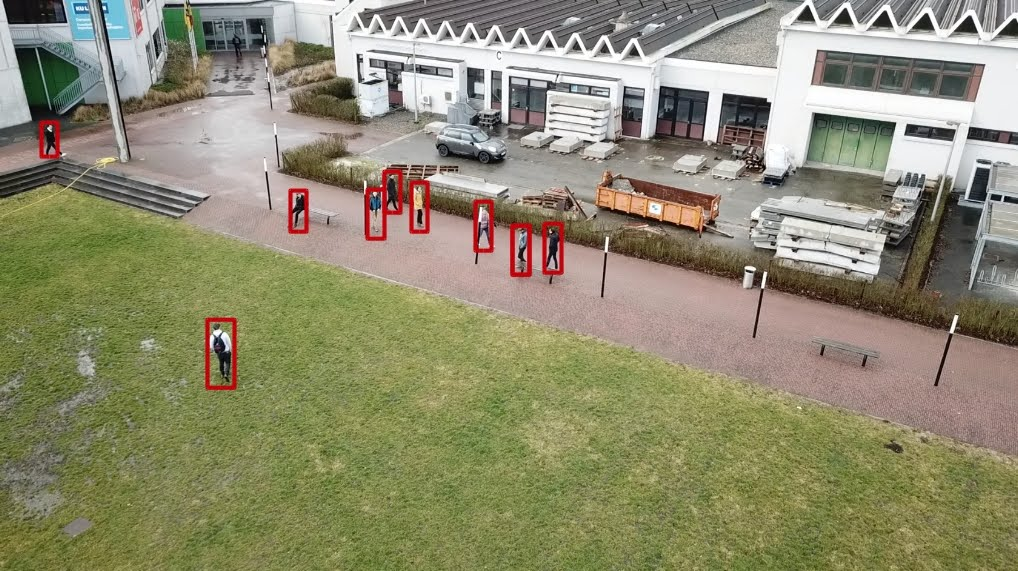
\includegraphics[width=0.56\linewidth]{3-visdrone-example}
    \caption{Примеры изображений SDD и VisDrone наборов данных} \label{sdd-visdrone-example}
\end{figure}


В силу специфичности решаемой задачи, пришлось самостоятельно формировать и организовывать сбор обучающей выборки с необходимыми нам фотографиями. Для решения этой задачи были привлечены добровольцы из различных ПСО, а также, разработаны методические материалы по сбору и разметке данных \cite{lib-lacmus-wiki-images}\cite{lib-lacmus-wiki-label}.

В результате был получен уникальный в своем роде набор данных, получивший в последствии название Lacmus Drone Dataset (LaDD) \cite{lib-ladd}. LaDD состоит из 1431 фотографии и имеет формат аннотирования Pascal VOC \cite{lib-pascal} с одним классом "Pedestrian" (пешеход). Dataset также является открытым и распространяется по лицензии GNU GPL v3. В его создании приняло участие множество ПСО из различных регионов России (Москва, Саратов, Ямал, Крым, Калининград и др). Таким образом, удалось достичь высокого разнообразия природных условий и, как следствие, и обучающей выборки. Ниже приведен пример фотографии:

\addimghere{3-ladd-example}{1}{Московская область, осень 2019, бурелом, лежачий на боку человек}{ladd-example}

\clearpage % Постановка задачи
\section{Архитектуры нейросетевых детекторов}\label{sect-4}

Различают несколько типов нейросетевых детекторов: One-stage и two-stage \cite{lib-detector-types}.

Two-stage -- более старый подход детекции. Он состоит из двух этапов. Сначала генерируются области, которые соответствуют искомым объектам. Ненужные области отсеиваются с помощью классификатора, например AlexNet \cite{lib-alexnet}. Такой подход является довольно точным, но не эффективен как по скорости, так и по памяти. Ярким примером такого подхода могут послужить такие архитектуры как: R-CNN и Faster R-CNN \cite{lib-rcnn}.

One-stage -- более быстрый и состоит из одного шага. Сначала изображение попадает в backbone -- базовую сверточную нейронную сеть. Сигналы из разных ее уровней пробрасываются в сеть трансформирующую признаки, а затем, производится классификация и детекция. Представителями этого подхода являются: SSD \cite{lib-ssd}, YOLO \cite{lib-yolo}, RetinaNet \cite{lib-retinanet}, TTFNet \cite{lib-ttfnet}.

\subsection{Выбор подходящего детектора}

В качестве кондидатов мною были выбраны лучшие архитектуры за последние 7 лет. Отбор производился на основе соремнований для задачи детекции MS COCO. Ниже приведен список этих типов СНС:
\begin{itemize}
    \item MobileNet-v3 + SSD -- one-stage детектор симейства SSD с MobileNet (v3) в качестве backbone;
    \item YOLO-v4 (Darknet-53) -- one-stage детектор симейства YOLO v4 с Darknet-53 в качестве backbone;
    \item EfficientDet-D3 -- one-stage детектор симейства Efficientdet с EfficientNet-B3 в качестве backbone;
    \item TTFNet-53 -- one-stage детектор симейства TTFNet с Darknet-53 в качестве backbone;
    \item RetinaNet (Resnet-50) -- one-stage детектор симейства RetinaNet с Resnet-50 в качестве backbone;
    \item Faster RCNN -- two-stage детектор симейства Faster RCNN.
\end{itemize}

Все перечисленные выше кондидаты были поставлены в одиноковые условия и обучались по одному алгоритму:
\begin{itemize}
    \item СНС инициализировалась со случайными весами;
    \item СНС обучалась на выборке MS COCO (100 эпох);
    \item Обученная на предыдущем шаге СНС дополнительно обучалась на LaDD и VisDrone (10 эпох).
\end{itemize}

Результаты эксперемента приведены в таблице \ref{leaderboard-table}.

\begin{table}[H]
    \caption{Сравнение различных архитектур детекторов}\label{leaderboard-table}
    \begin{tabular}{|p{4cm}|p{3cm}|p{3cm}|p{5cm}|}
    \hline
    {Тип} & {mAP (LaDD)} & {mAP (VisDrone)} & {Время обработки изображения (Tesla v100)} \\
    \hline
    MobileNet-v3 + SSD & 0.46 & 0.12 & 100 мс \\
    \hline
    YOLO-v4 (DarkNet-53) & 0.52 & 0.15 & 270 мс \\
    \hline
    EfficientDet-D3 & 0.66 & 0.23 & 400 мс \\
    \hline
    TTFNet-53 & 0.65 & 0.21 & 300 мс \\
    \hline
    RetinaNet (ResNet-50) & 0.71 & 0.25 & 300 мс \\
    \hline 
    Faster RCNN & 0.72 & 0.24 & 500 мс \\
    \hline
    \end{tabular}
  \end{table}

  Из эксперимента видно что по совокупности точности и скорости работы лучше всего справляется с детекцией RetinaNet. Также превосходтсво этой архитектуры подтверждает еще одно исследование. В нем сравнения СНС проводились на выборке Stenfird Drone Dataset (SDD) в которой содержится около 1 миллиона изображений снятых с БПЛА в кампусе Стенфордского Университета. Некоторые результаты этого исследования приведены в таблице \ref{leaderboard-table-sdd}.

  \begin{table}[H]
    \caption{Сравнение различных архитектур детекторов на выборке SDD}\label{leaderboard-table-sdd}
    \begin{tabular}{|p{7cm}|p{5cm}|}
    \hline
    {Тип} & {mAP (SDD)} \\
    \hline
    SSD (ResNet-50) & 0.80 \\
    \hline
    Faster RCNN (ResNet-50) & 0.83 \\
    \hline
    RetinaNet (Resnet-50) & 0.85 \\
    \hline
    \end{tabular}
  \end{table}

  Из вышеперечисленных исследований следует, что RetinaNet в сравнении с другими архитектурами обладает высокой точностью и скоростью работы и ее можно применять для решения задач детектирования объектов по снимкам с БПЛА.


\clearpage % Постановка задачи
\subsection{Устройство RetinaNet}\label{sect-5}

Архитектура RetinaNet, взятая за основу для моего исследования, состоит из ряда основных частей. Каждая из них выполняет определенную функцию:
\begin{itemize}
    \item backbone (или базовая сеть) -- необходима для извлечения тензора признаков (feature extraction) из входного изображения. В качестве нее может быть выбран один из нескольких вариантов СНС таких как: ResNet, EfficientNet, MobileNet и прочие;
    \item Feature Pyramid Network (FPN) -- пирамидальная СНС, необходима для трансформации признаков \cite{lib-fpn}. Она объединяет карты признаков приходящих как с верхних, так и с нижних уровней базовой СНС, так как первые обладают низкой обобщающей способностью (receptive field) при большей размерности, а последние -- наоборот;
    \item Classification Subnet Network (подсеть классификации) -- необходима для извлечения информации о классах. Классификация происходит для каждого уровня пирамиды, затем результаты фильтруются;
    \item Regression Subnet Network (подсеть регрессии) -- необходима для извлечения информации о положении объекта. Регрессия также происходит для каждого уровня пирамиды, затем результаты фильтруются;
    \item Блок пост обработки -- представляет собой набор алгоритмов для фильтрации предсказаний СНС. Как правило, здесь применяются такой алгоритм как NMS (Non Maximum Suppression) \cite{lib-nms}.
\end{itemize}

Ниже приведена общая архитектурная схема RetinaNet:

\addimghere{5-retinanet-architecture}{1}{Архитектурная схема RetinaNet}{retinanet-architecture}

Рассмотрим каждую из частей RetinaNet подробнее.

\subsection{Backbone}

Как говорилось выше, базовая сеть может быть реализована по разному. Так как от ее выходных признаков зависят предсказания остальных частей детектора -- необходимо выбрать наиболее подходящую архитектуру для backbone-СНС.

Для этого были проанализированы исследования последних лет. В качестве сравнительных характеристик были выбраны accuracy и времени работы, а в качестве обучающей выборки -- ImageNet. На изображение ниже приведены результаты исследований:

\addimghere{5-1-resnet-benchmark}{1}{Сравнение различных СНС на ImageNet 2020}{retinanet-architecture}

Представленная еще в 2015 году Microsoft Research архитектура ResNet \cite{lib-resnet} оказалась настолько удачной, что и по сей день периодически ставит рекорды в области распознавания изображений. Рассмотрим семейство архитектур ResNet подробнее.

Ее успех заключается в применении Residual блоков. С ростом числа слоев в нейронной сети все острее встает проблема паралича нейронной сети -- из-за обратного распространения ошибки градиент от слоя к слою постоянно уменьшается. В результате более глубокие слои перестают обучаться и как следствие качество распознавания падает:

\addimghere{5-1-cnn-back-propagation-paralysis}{0.8}{Увеличение колличества слоев дает ходший результат}{back-propagation-paralysis}

Основная идея ResNet заключается в том, чтобы ввести так называемое "соединение с пропусками" (Skip Connection), которое пропускает один или несколько уровней, как показано на рисунке ниже:

\addimghere{5-1-residual-block}{0.6}{Residual блок}{residual-block}

Благодаря Residual блокам, градиент не уменьшается, а слои СНС можно объединять в длинные последовательности, увеличивая как обобщающую способность, так и точность такой сети:

\addimghere{5-1-resnet-training-results}{1}{Кривые обучения ResNet (справа) с 18 и 34 слоями в сравнении с аналогичной СНС без residual обоков (слева)}{residual-block}
\subsection{Feature Pyramid Network} \label{sect-5-2}

FPN состоит из нескольких частей (рис. \ref{fpn-arch}): восходящей (bottom-up) и низходящей (top-down) пирамид, а также боковых соединений (lateral connections). Рассмотрим подробнее каджую часть.

\addimghere{5-2-fpn-arch}{0.8}{Архитектура FPN}{fpn-arch}

Восходяая пирамида -- есть некоторая последовательность светросных слоев, расзмерность которых уменьшается, извлекающяя признаки из входного изображения. В нашем случае это базовая сеть (ResNet50). Стоит отметить, что по с ростом уровней пирамиды увеличивается число информации, содержащиеся в каждос супер-пикселе сверточного слоя (receptive fild), но вместе с тем уменьшается размерность выходного тензора. 
Из-за этого факта bottom-up пирамида обладает уязвимостью -- важные призноки, особенно если обьект небольной, могут потерятся при перекрытии объекта (человек прикрыт травой) а конечные обьекты имеют размер в несколтко супер-пикселей (рис. \ref{fpn-distribution}). Как следистве СНС будет работать нестабильно, а колличество ошибок 1 и 2 рода возрастет. 

\addimghere{5-2-fpn-distribution}{0.6}{Внутреннее представление человека на одном из верхних уровней FPN}{fpn-distribution}

Некоторые пути решения этой проблемы будут рассмотрены в следующих разделах, а сконцентрируемся на устройстве FPN.

Низходящая пирамида -- напротив представляет собой полследовательность всерточных слоев размерность которых увеличивается по мере спуска сигнала. На каджом шаге размерность карт признаков возрастает в 2 раза, недостающие признаки выбираются методом ближайших соседей ((рис. \ref{fpn-top-down-knn})). Начальные уровни top-down пирамиды имеют такую же размерность что и верхние уровни bottom-up пирамиды, а размеры последних -- наоборот соответствуют первым уровням backbone-сети.

\addimghere{5-2-fpn-top-down-knn}{0.5}{Увеличение размерности признаков методом ближайшего соседа}{fpn-top-down-knn}

В добавок, между пирамидами в FPN существуют и боковые соединения. Благодаря ми, признаки соответствующих слоёв поэлементно складываются, причём карты из bottom-up пирамиды проходят через свёртку $1 \times 1$ (рис. \ref{fpn-connections}).

\addimghere{5-2-fpn-connections}{0.6}{Устройство боковых соеденений}{fpn-connections}

Уровни пизходящей пирамиды принято обозначать как $P_1, P_2, ..., P_n$, притом каждый $i$ уровень top-down пирамиды соответст сответствует $i$-му уровню bottom-up пирамиды $C_1, C_2, ..., C_n$. Кллличество $P$ уровней может быть меньше от колличества уровней $С$. Тогда уровни низходящей пирамиды могут быть сдвинуты на некоторый шаг. Так оригинальная FPN имеет конфигурацию с пятью уровнями $P_3...P_7$. На изображении ниже приведен пример FPN сети с кофигурацией $P_3...P_5$:

\addimghere{5-2-fpn-p3-p5}{0.8}{Архитектура FPN c $P_3...P_5$ уровнями}{5-2-fpn-p3-p5}
\subsection{Anchor boxes}

Анкерные или якорные рамки (anchor boxes) впервые были предложены в архитектуре Faster RCNN и затем получили свое распространение на многие современные архитектуры детекторов таких как YOLO или RetinaNet. 

Предположим, что СНС сворачивает исходное изображение до тензора размерности $3 \times 3$. Таким образом, в каждом супер-пикселе выходного тензора содержится информация о некоторой области исходного изображения. Тогда можно предположить размеры объекта попадающего в такой супер-пиксель (рис. \ref{anchor-boxes}). Эти размеры, их количество и ориентация и называются анкерными рамками (т.е. рамками "привязанными" к супер-пикселю). Для RetinaNet каждый супер-пиксель имеет анкоры с соотношениями сторон $2:1, 1:1, 1:2$ и размерами $2^0, 2^{\frac{1}{3}}, 2^{\frac{2}{3}}$ (и того 9 штук). При обучении модели для каждого объекта подбираются в наиболее подходящие анкоры. Если $IoU$ рамки больше 0.5, то она считается верной, а если меньше 0.4 -- ложной. В случаях когда $IoU \in [0.4 .. 05]$ anchor box будет проигнорирован для обучения.

\addimghere{5-3-anchor-boxes}{0.6}{Аnchor boxes}{anchor-boxes}
\subsection{Подсети классификации и регрессии}

Classification и regression subnet получают на вход признаки из нисходящей пирамиды FPN и выдают предсказания о классе и местоположении объекта. 

В подсети классификации сигнал сперва проходит через 4 сверточных слоя с размерностью $[3 \times 3]$, с 256 фильтрами и со стоящей после ReLU активацией. Таким образом, в каждом convolution слое формируется тензор размера $[h \times W \times 256]$ (256 карт признаков). Затем, сигнал снова проходит через сверточный слой $[3 \times 3]$, но уже с $K \times A$ фильтрами и сигмоидальной активацией. В результате, на выходе этой сети формируется вектор длиной $K \times A$, где $K$ -- количество разных классов (в нашем случае только один класс -- это Pedestrian), $A$ -- количество анкерных рамок. Подсеть для каждого анкера выдает one-hot вектор, где позиция числа 1 соответствует номеру класса для каждого анкера к которому модель отнесла объект.

В подсети регрессии первые 4 слоя эквивалентны соответствующим слоям в classification subnet. Затем, идет свертка,  $[3 \times 3]$ формирующая $4 \times A$ карт признаков. После чего, аналогично классификационной подсети, формируется вектор длинны $4 \times A$. Таким образом, подсеть позволяет уточнить 4-компонентный вектор координат анкера под реальный размер объекта: $(\Delta x_{min}, \Delta y_{min}, \Delta x_{max}, \Delta y_{max})$.
\subsection{Функция потерь}

Отметим, что функция потерь (loss function) складывается из двух компонент: ошибки регрессии и классификации (формула \ref{eq-1}).

\begin{equation}\label{eq-1}
    L = \lambda L_{reg}+L_{cls}
\end{equation}
где:
\begin{itemize}
    \item $L$ -- функция потерь RetinaNet;
    \item $L_{reg}$ -- ошибки регрессии;
    \item $L_{cls}$ -- ошибки классификации;
    \item $\lambda$ -- коэффициент усиления, определяющий соотношение между потерями.
\end{itemize}

Рассмотрим из чего складываются потери регрессии. Мы знаем, что каждому объекту ставится в соответствии анкерная рамка. Пусть $G$ -- целевой (ground truth) объект, а $A$ -- анкер. Тогда, сопоставив объекты и anchor box-ы получим $s$ пар: $(G_i, A_i), i=1..s$.

Заметим, что для каждого анкера regression subnet отдает вектор, показывающий разницу между границами якорной рамки и объекта: $(\delta x_{min}, \delta y_{min}, \delta x_{max}, \delta y_{max})$.  Подсчитав действительное расстояние между анкером и границами объекта  $(\Delta x_{min}, \Delta y_{min}, \Delta x_{max}, \Delta y_{max})$ и сравнив его с результатами работы подсети, вычислим потери регрессии:
$$
L_{reg} = \sum_{i, j} smooth_{L1}(\delta_{ij}-\Delta_{ij})
$$
где:
\begin{itemize}
    \item $\delta_{ij}$ -- прогнозируемое расстояние между anchor box-ом и границами объекта;
    \item $\Delta_{ij}$ -- реальное расстояние между anchor box-ом и границами объекта;
    \item $i \in {x, y},\ j \in {min, max}$;
    \item $smooth_{L1}(x) = \begin{cases}\frac{1}{2}x^2, & \mid x\mid < 0\\\mid x\mid - \frac{1}{2}, & x \geq 0\end{cases}$
\end{itemize}

Для потерь классификации используется функция Focal Loss \cite{lib-focal-loss}:
$$
L_{cls} = -\sum_{i=1}^K \alpha_i \cdot log(p_i)(1-p_i)^\gamma
$$
где:
\begin{itemize}
    \item $K$ -- количество классов;
    \item $p_i$ -- вероятность с которой класса $i$ был предсказан;
    \item $\gamma$ -- фокальный коэффициент;
    \item $\alpha_i$ -- коэффициент усиления класса $i$ (в нашем случае мы имеем только один класс и $\alpha$ = 1).
\end{itemize}

Данная функция есть усовершенствование функцией кросс-энтропии \cite{lib-focal-loss}, где от модели требуется высокая степень "уверенности" и влияние часто встречающихся классов возрастает. В Focal Loss это влияние, наоборот, снижается, а наибольший вклад при обучении весов RetinaNet оказывают редко встречающиеся объекты. Делается это за счёт множителя $(1-p_i)^\gamma$, а также параметров $\alpha_1$ и $\gamma \in(0, \infty)$. Графики функций focal и cross entropy представлены на рисунке ниже:

\addimghere{5-5-focal-loss}{0.8}{Графики focal loss и cross entropy}{focal-loss}

Стоит отметить, что во время обучения, большая часть объектов, обрабатываемых классификатором, является фоном, который является отдельным классом. Поэтому может возникнуть проблема, когда нейросеть обучится определять фон лучше, чем другие объекты. Такая несбалансированность очень характерно для решаемой задачи детектирования пропавших людей. По этому, в качестве функции потерь была выбрана Focal Loss.
\subsection{Пост-обработка}

Зачастую получается так, что СНС отдает на выходе несколько прогнозов указывающих на один и тот же объект. В этом случае такие предсказания следует отфильтровать, выбрав наилучшие (рис. \ref{nms}). Однако, при фильтрации стоит учитывать случай, когда на изображении два разных объекта одного класса могут находиться рядом, и их ограничивающие рамки могут пересекаться. Эта задача решается на этапе пост-обработки с помощью алгоритма Non-Maximum Suppression (NMS).

\addimghere{5-6-nms}{0.8}{Пример работы NMS}{nms}

На вход NMS принимает набор bounding box-ов для одного класса и порог, задающий величину максимального пересечения между ними. Ограничивающие рамки сортируются по уверенности (accuracy) и кладутся на стек. В первом цикле со стека берется очередная гипотеза. Затем, во вложенном цикле со стека берется вторая гипотеза. Если между двумя гипотезами IoU больше заданного порога, то вторая гипотеза отбрасывается. Алгоритм продолжает работу до тех пор пока не переберет все пары ограничивающих рамок.

Код алгоритма может выглядеть так:

\lstinputlisting[numbers=left]{inc/scripts/nms.py} % Постановка задачи
%\input{inc/0-conclusion} % Заключение
%\input{inc/0-bibliography} % Библиографический список

% Приложения
%\vspace*{\fill}
\centering{\uppercase{Приложение}}
\vspace*{\fill}

\clearpage

\appsection{Приложение А}
\centering{\uppercase{Исходный код интерфейсов системы модулей и модуля LacmusRetinanetPlugin.DirectML}}
\vspace{\baselineskip}

\lstinputlisting[numbers=left]{inc/scripts/lacmus-plugins/LacmusPlugin/IObjectDetectionPlugin.cs}

\lstinputlisting[numbers=left]{inc/scripts/lacmus-plugins/LacmusPlugin/IObjectDetectionModel.cs}

\lstinputlisting[numbers=left]{inc/scripts/lacmus-plugins/LacmusPlugin/IObject.cs}

\lstinputlisting[numbers=left]{inc/scripts/lacmus-plugins/LacmusPlugin/Version.cs}

\lstinputlisting[numbers=left]{inc/scripts/lacmus-plugins/LacmusPlugin/Enums/InferenceType.cs}

\lstinputlisting[numbers=left]{inc/scripts/lacmus-plugins/LacmusPlugin/Enums/OperatingSystem.cs}

\lstinputlisting[numbers=left]{inc/scripts/lacmus-plugins/LacmusRetinanetPlugin.DirectML/Model.cs}

\lstinputlisting[numbers=left]{inc/scripts/lacmus-plugins/LacmusRetinanetPlugin.DirectML/Plugin.cs}

\clearpage % Исходный код скрипта DDoS Deflate
%\input{inc/b-app} % Руководство пользователя

%\includepdf{act} % Акт внедрения

\end{document}
%%% Конец документа